In this section we investigate how and whether the graph-based approaches improve the classification score when combined with text-based approaches.
This is arguably the most interesting question since it will show the usefulness of concept maps in text classification.

For the text features we vectorized the text with Bag-Of-Word approaches, namely a simple term frequency count and augmented by Tfidf.
Here, we evaluated both uni-grams and bi-grams by cross-validation, then we chose the best performing variant to evaluate on the test set.
For the graph features we used the Weisfeiler-Lehman algorithm since it is able to create feature map $\phi(G)$ for the graphs.
These feature maps can easily be concatenated with the text features.
For other graph kernels where an explicit feature map $\phi(G)$ can not be calculated, in order to combine graph- and text features, we would have needed to create a combined kernel that takes both text- and graph features into account and calculate a gram matrix.
The interpretability of this approach would be far lower since both graph- and text-features would be merged together in a single number which inhibits to distinguish the relative importance of the text- and graph features after creating the gram matrix.
In Table \ref{table:results_comparison_combined} we see the classification scores for the combined features for both co-occurrence graphs and concept maps.
We also report the scores of different Weisfeiler-Lehman extensions and graph pre-processing steps, eg. splitting multi-word labels.
The details of these approaches will we introduced in the answers for the next questions.

In the results we can see that the classification performances of the text-only and and combined approaches are comparable.
On some datasets, the combined approach is slightly better than the text-only approach.
Yet, under the permutation test, these differences are not significant.
Interestingly, the co-occurrence graphs with their relatively simple structure often perform the best when combined with text features.
However, on other datasets, their performance is not as good as the scores of text-only- or combined with concept maps approaches.
Another interesting observation concerns the different WL extensions and graph-preprocessing steps we devised for concept maps.
Here, we see only minor improvement or even lower performance than with the combined approach.
When doing graph-only classification, on the other hand, we see high improvements over the plain version, ie. plain WL and no graph pre-processing.
For instance, one approach, which linearizes the graph into text and subsequently uses uni-gram Tfdif Bag-Of-Words to vectorize the text, consistently results in lower classification performance when combined with the conventional text approach.
On the other hand, when doing graph-only classification, linearizing the graph into text actually consistently resulted in the best scores.
So, while ignoring the structure in graph-only classification has shown the best performance, on the combined approach, it performed worse than other extensions or even plain WL.
This observation can also be seen with other extensions, yet not as distinguished.
All these observations highlight the importance of carefully selecting the used graph kernels.
Using different variants of the Weisfeiler-Lehman graph kernel, for example, resulted in greatly varying performance on different datasets.
Also, the performances on graph-only classification differ from the performance when combining text- and graph features.

To better understand the classification performance when combining text- and graph features, we also train a one-layer neural network\footnote{Implementation: \url{http://scikit-learn.org/stable/modules/generated/sklearn.linear_model.SGDClassifier.html}} with the combined features using stochastic gradient descent. After training we investigate the weights.
The weights, or coefficients, for each input feature are an indicator for the importance of that input feature.
Thus we can look at weights for the text features and compare them to weights for graph features.
This gives us an insight into the relative importance of text- and graph features.
In Figure \ref{fig:coefs_example_one_layer} we show an example of an one-layer neural net.
For our purposes, we do not look at single features, or input neurons, but on a range of features, namely the text and graph feature ranges since, in our case, the text- and graph features are concatenated.

\begin{figure}[htb!]
    \centering
    {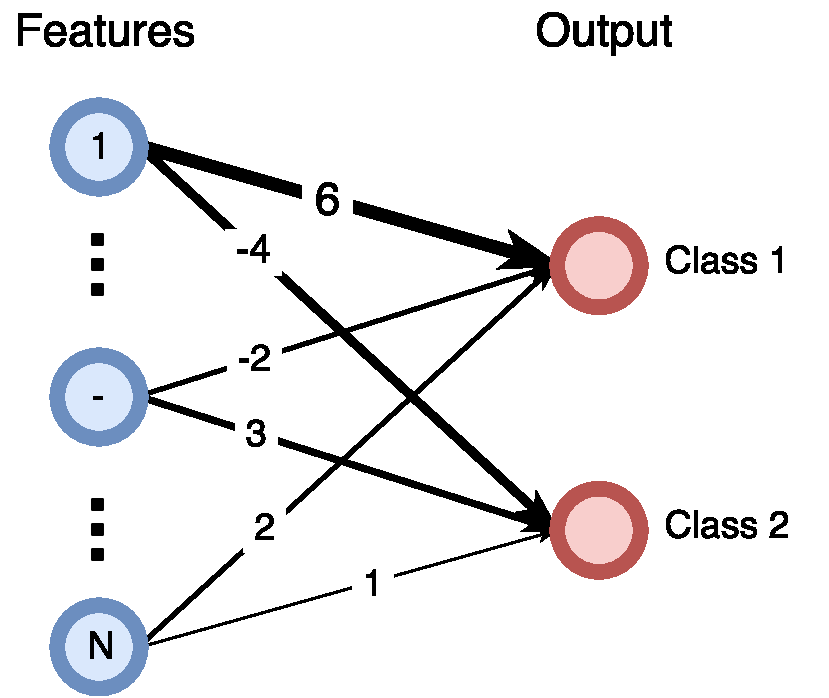
\includegraphics[width=0.5\linewidth]{assets/figures/coefs_example.pdf}%
        \caption[Example: One-layer neural net]{%
            Example of an one-layer neural net. The numbers on the line from input features to the output are weights.
            We examine these weights for single features to gain an insight into the importance the neural net assigned to a given feature. Since a feature contributes to all output neurons, we look at the sum of its absolute weights. Eg. for \textit{Feature 1} the sum of the absolute weights would be $|6| + |-4| = 10$ and for \textit{Feature N} it is $|2| + |1| = 3$, which gives us the hint that \textit{Feature 1} might be more important for the classification result than \textit{Feature N}.
            This analysis presupposes that the feature magnitudes, ie. the values of features, are normalized or - roughly speaking - in the same range on average, eg. \textit{Feature 1} does not take values between $[100, 200]$ while \textit{Feature N} takes values from $[0, 1]$, instead both feature values are roughly in the same range.
        }%
        \label{fig:coefs_example_one_layer}}
\end{figure}

Figure \ref{fig:combined_coefs_l1_l2_regularization} then shows an example of a weight analysis for the \textit{ng20} dataset and for two regularizations, namely \textit{L1} and \textit{L2}.

Both regularization terms are used to discourage ``big" weights, effectively forcing the training algorithm to chose important features to generalize the data instead of over-fitting the data.
While both \textit{L1} and \textit{L2} regularization discourage big weights, \textit{L1} penalizes small weights harder than \textit{L2}, leading to more zero coefficients \cite[p.~13]{Hastie2009}.
Therefore, the selection of important features is enforced more with \textit{L1} regularization.
We leverage this phenomenon to analyze how important the features, graph and text, are for classification.
When looking at the absolute sum of the weights of the trained one-layer neural net, we discover that using \textit{L1} regularization results in the text features becoming more important than graph features for classification.
While the difference of absolute sums of the coefficients does not seem especially high, it has to be noted that graph features are approximately only half as dense as text features.
Thus the contribution by graph features to the end result is even lower than the neural net coefficients indicate.

\begin{figure}[htb!]
    \centering
    {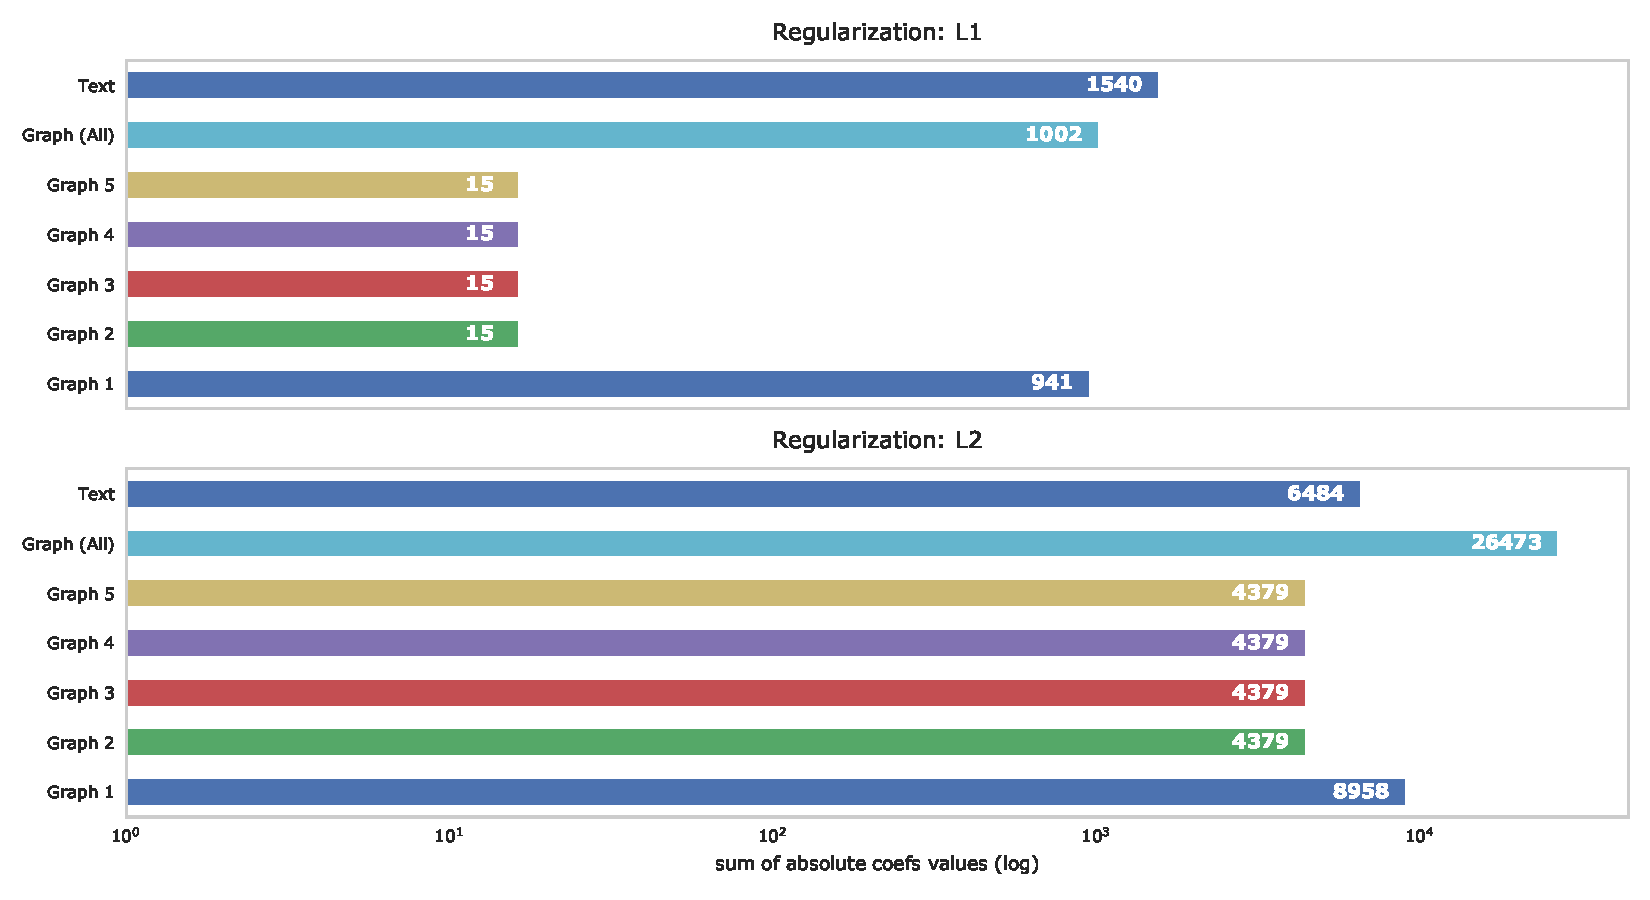
\includegraphics[width=\linewidth]{assets/figures/combined_coefs_l1_l2_regularization.pdf}%
        \caption[Statistics: Histogram of the trained weights of a one-layer neural net]{%
            Histogram of the trained one-layer neural net weights. The neural net was trained on the concatenated graph- and text features.
            Higher values indicate higher importance.
            \textit{Graph (All)} stands for the sum of all graph feature weights, while the \textit{Graph $N$} stand for the individual Weisfeiler-Lehman iterations.
            Higher iterations of WL take a bigger neighborhood into account.
            Dataset: \textit{ng20}.
        }%
        \label{fig:combined_coefs_l1_l2_regularization}}
\end{figure}

Another interesting result of this weight analysis is the importance the neural net assigns to different Weisfeiler-Lehman iterations. In our example, we chose $h = 5$ for our WL iterations. The higher the iteration, the bigger the neighborhood that is considered by WL.
When looking at the importance of the first iteration and \textit{L1} regularization, \textit{Graph 1} in Figure \ref{fig:combined_coefs_l1_l2_regularization}, we see that while the neural net nearly discourages all higher WL iterations by assigning low weights, it assigns higher importance to the first iteration of WL.
The first iteration of WL takes only the immediate neighborhood into account, therefore matches are far more probable than matches in higher iterations.
In our example in Figure \ref{fig:combined_coefs_l1_l2_regularization}, \textit{L1}- outperformed \textit{L2} regularization by a high margin, approximately 7\% difference in the \textit{F1} macro score.
However, it has to be noted that no hyper-parameter tuning was performed and only a simple train-/test split was used.

\begin{table}[htb!]
\centering
\begin{tabular}{ll|cccc|c|c}
	\toprule
	& & \multicolumn{6}{c}{F1 macro} \\
	&  & \multicolumn{4}{c|}{Concept Map} & Co-Occurrence &  Text \\
	&  &   WL & Split + WL & To-Text & Infreq. + WL &  WL &    \\
	\midrule
ling-spam & Single & 0.816 & 0.913 & 0.934 & 0.803 & 0.987 & \textbf{0.990} \\
& Combined & \textbf{0.990} & 0.986 & 0.980 & \textbf{0.990} & 0.984 &\\
\midrule
ng20 & Single & 0.419 & 0.574 & 0.622 & 0.357 & 0.593 & \textbf{0.781} \\
& Combined & \textbf{0.791} & 0.737 & 0.756 & 0.781 & 0.672 &\\
\midrule
nyt\_200 & Single & 0.744 & 0.846 & 0.899 & 0.774 & 0.881 & \textbf{0.921} \\
& Combined & \textbf{0.917} & 0.891 & 0.904 & 0.888 & 0.875 &\\
\midrule
r8 & Single & 0.677 & 0.860 & 0.892 & 0.633 & 0.890 & \textbf{0.921} \\
& Combined & 0.921 & 0.929 & \textbf{0.931} & 0.929 & 0.914 &\\
\midrule
review\_polarity & Single & 0.609 & 0.715 & 0.737 & 0.607 & 0.785 & \textbf{0.877} \\
& Combined & 0.870 & 0.837 & 0.850 & \textbf{0.880} & 0.855 &\\
\midrule
rotten\_imdb & Single & 0.635 & 0.780 & 0.828 & 0.551 & 0.825 & \textbf{0.886} \\
& Combined & 0.885 & 0.877 & 0.883 & 0.890 & \textbf{0.910} &\\
\midrule
ted\_talks & Single & 0.244 & 0.413 & 0.359 & 0.364 & 0.443 & \textbf{0.464} \\
& Combined & \textbf{0.481} & 0.433 & 0.436 & 0.468 & 0.442 &\\
	\bottomrule
\end{tabular}
\caption[Results: Combined text- and graph features]{Classification results for combined graph- and text features classification.
\textit{Split} stands for the WL extension where the multi-word labels are split, see answer to Question \ref{subquestionanswer:question:multi_labels}.
\textit{To-Text} converted the graph back to text, then a classifical Tfidf-BoW approach was used, see answer to Question 3.
\textit{Infreq.} is the WL extension where infrequent nodes are ignored, see answer to Question 7.
No significant improvement of the combined approach was found upon the text-only features, under the permutation test.
}%
\label{table:results_comparison_combined}
\end{table}

\answersummary{
    When combining the graph- and text features we do not achieve no significantly higher classification scores and even observe a degradation.
    Examining the weights of one-layer neural net shows us that, when training on combined text- and graph feature, graph features get lower absolute weights assigned.
    A possible explanation is that the graph features are not as important for the combined text- and graph feature classification.
}